\documentclass[border=10pt]{standalone}
\usepackage{tikz}
\usetikzlibrary{arrows.meta, shapes, calc}

\begin{document}

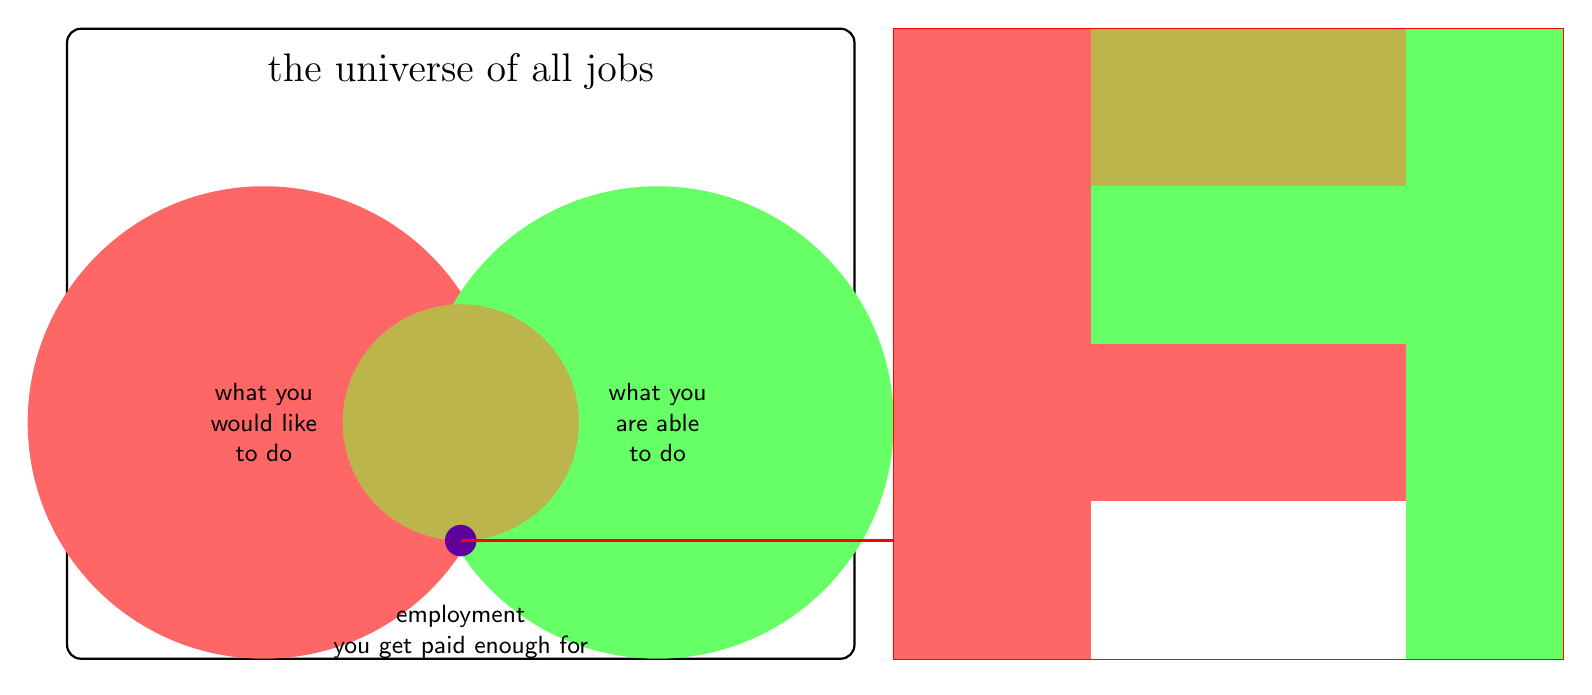
\begin{tikzpicture}[scale=1.0, every node/.style={font=\sffamily\small}]

% Left Panel: Venn Diagram
\draw[thick, rounded corners=5pt] (0,0) rectangle (10,8);
\node[anchor=north, font=\Large] at (5,7.8) {the universe of all jobs};

% Left Circle: "what you would like to do"
\fill[red!60] (2.5,3) circle (3cm);
\node[align=center] at (2.5,3) {what you\\would like\\to do};

% Right Circle: "what you are able to do"
\fill[green!60] (7.5,3) circle (3cm);
\node[align=center] at (7.5,3) {what you\\are able\\to do};

% Intersection (olive green)
\fill[olive!60] (5,3) circle (1.5cm);

% Tiny purple circle at the bottom of intersection
\fill[blue!50!purple] (5,1.5) circle (0.2cm);
\draw[thick, red] (5,1.5) -- (10.5,1.5); % Line to right panel

% Label for employment
\node[align=center, anchor=north] at (5,0.8) {employment\\you get paid enough for};

% Right Panel: Zoomed-in View
\draw[thick, red] (10.5,0) rectangle (19,8);

% Large circle in right panel
\draw[ultra thick, black] (14.5,4) circle (3cm);

% Divide circle into 4 quadrants
\draw[ultra thick, black] (14.5,4) -- (17.5,4); % right
\draw[ultra thick, black] (14.5,4) -- (11.5,4); % left
\draw[ultra thick, black] (14.5,4) -- (14.5,7); % top
\draw[ultra thick, black] (14.5,4) -- (14.5,1); % bottom

% Fill quadrants
\fill[blue!60] (14.5,4) -- (17.5,4) arc (0:90:3) -- cycle;
\fill[blue!40] (14.5,4) -- (17.5,4) arc (0:-90:3) -- cycle;
\fill[violet!80] (14.5,4) -- (11.5,4) arc (180:90:3) -- cycle;
\fill[blue!50!purple!80] (14.5,4) -- (11.5,4) arc (180:270:3) -- cycle;

% Label "perfect job"
\node[align=center] at (15.5,5.5) {perfect\\job};
\fill[black] (15.5,5.5) circle (0.05cm);

% Background color regions
\fill[red!60] (10.5,0) rectangle (13,8);
\fill[green!60] (17,0) rectangle (19,8);
\fill[olive!60] (13,8) rectangle (17,6);
\fill[green!60] (13,6) rectangle (17,4);
\fill[red!60] (13,4) rectangle (17,2);
\fill[white] (13,2) rectangle (17,0);

\end{tikzpicture}

\end{document}